\documentclass[UTF8,a4paper,11pt]{ctexart}

\usepackage[margin=2.2cm]{geometry}
\usepackage{amsmath,amssymb,bm}
\usepackage{booktabs}
\usepackage{graphicx}
\usepackage{hyperref}
\usepackage{enumitem}
\usepackage{caption}

\hypersetup{colorlinks=true,linkcolor=blue,citecolor=blue,urlcolor=blue}
\setlist[itemize]{leftmargin=2em}
\setlength{\parindent}{2em}
\setlength{\parskip}{0.25em}

\title{密集同频 LEO Follower 网络的干扰扩展结果分析}
\author{Numerical study report for the interference-extension branch}
\date{\today}

\begin{document}
\maketitle

\section{实验设置}

本报告基于复现版 Table I 默认参数，并把网络从噪声受限假设扩展为同频全复用下行网络。
典型用户由最近 leader cluster 服务；服务集群的 leader 和 followers 是期望信号源；
所有非服务 clusters 中可见的 leaders 与 followers 都作为地面同频干扰源。Monte Carlo
实验使用固定随机种子，并在 cluster rate 图中给出 95\% 置信区间；二维扫描图采用
均值干扰近似，以便快速比较 $N_{\rm L}$--$N_{\rm F}$ 参数面。

需要强调的是，这里的“干扰扩展”不是原论文图 2--8 的替代版本，而是以复现项目为基线
提出的新研究场景。它回答的问题是：当网络变得密集并且各集群同频工作时，继续增加
followers 是否仍然可靠地提升整体网络性能。

\section{Fig.I1：平均干扰功率随网络密度变化}

\begin{figure}[htbp]
    \centering
    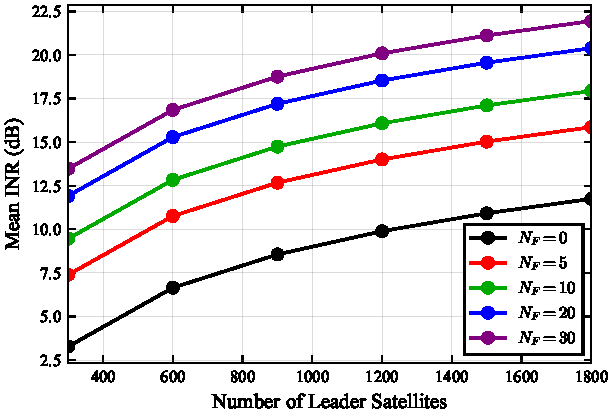
\includegraphics[width=0.78\linewidth]{../figures/interference/figI1_mean_inr.pdf}
    \caption{平均归一化干扰功率 INR 随 leader 数量和 follower 数量的变化。}
    \label{fig:i1}
\end{figure}

图 \ref{fig:i1} 说明平均 INR 对 $N_{\rm L}$ 和 $N_{\rm F}$ 都呈单调上升趋势。以
$N_{\rm L}=1500$ 为例，$N_{\rm F}=0$ 时平均 INR 约为 $10.92$ dB；当每个 leader
配置 $10$ 个 followers 时上升到 $17.11$ dB；当 $N_{\rm F}=30$ 时进一步上升到
$21.12$ dB。该结果直接对应理论推导中的
\[
    \bar I=(N_{\rm L}-1)\left(\bar I_{\rm L}^{(1)}
    +N_{\rm F}\bar I_{\rm F}^{(1)}\right),
\]
即 followers 的服务分集收益会伴随其他集群 followers 的线性干扰项一起出现。

\section{Fig.I2：SINR 覆盖概率退化}

\begin{figure}[htbp]
    \centering
    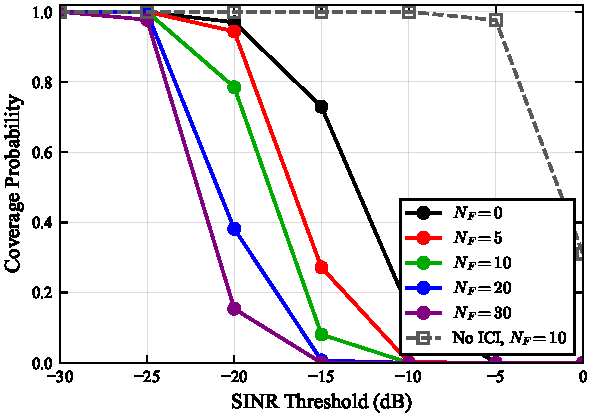
\includegraphics[width=0.78\linewidth]{../figures/interference/figI2_sinr_coverage.pdf}
    \caption{不同 follower 数量下的 cluster SINR coverage。虚线为关闭集群间干扰的基线。}
    \label{fig:i2}
\end{figure}

图 \ref{fig:i2} 展示了最明显的干扰受限转变。无集群间干扰且 $N_{\rm F}=10$ 时，
coverage 在 $-10$ dB 处仍约为 $1$，在 $-5$ dB 处约为 $0.976$。同频干扰打开后，
即使 $N_{\rm F}=0$，$-10$ dB coverage 也降至约 $0.153$；当 $N_{\rm F}=10$ 时，
$-15$ dB coverage 约为 $0.081$，$-10$ dB 已接近 $0$。这说明在密集同频部署下，
coverage 的瓶颈不再是单集群链路预算，而是可见区域中其他 cluster 的聚合干扰。

进一步增加 followers 会让曲线整体左移：$N_{\rm F}=30$ 时，coverage 在 $-20$ dB
也仅约 $0.154$，在 $-15$ dB 已降为 $0$。因此，若网络存在明确的 SINR 或 outage
约束，不能仅依据单集群无干扰速率来选择 follower 数量。

\section{Fig.I3：单集群速率的收益饱和}

\begin{figure}[htbp]
    \centering
    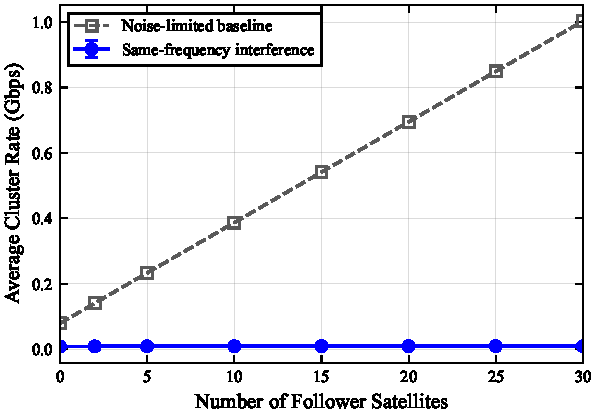
\includegraphics[width=0.78\linewidth]{../figures/interference/figI3_cluster_rate.pdf}
    \caption{平均 cluster rate 随 follower 数量变化：噪声受限基线与同频干扰模型对比。}
    \label{fig:i3}
\end{figure}

图 \ref{fig:i3} 中，噪声受限基线随 $N_{\rm F}$ 近似线性增长，从 $0.079$ Gbps
增长到约 $1.003$ Gbps。这与原复现图 6 的趋势一致，因为每个 follower 都提供新的
中继分支。相反，同频干扰模型下的平均 cluster rate 被压低在 $0.0083$--$0.0093$
Gbps 范围内，增加 followers 只能带来很小的边际改善。

这不是数值错误，而是同频全复用假设下的物理结果：服务集群得到更多 follower 分支，
但每个其他 cluster 也同步增加同数量的下行干扰源。因此，单集群平均速率没有像噪声
受限基线那样继续线性增长，而是很快进入干扰受限平台区。

\section{Fig.I4：全网吞吐的缓慢增长与代价}

\begin{figure}[htbp]
    \centering
    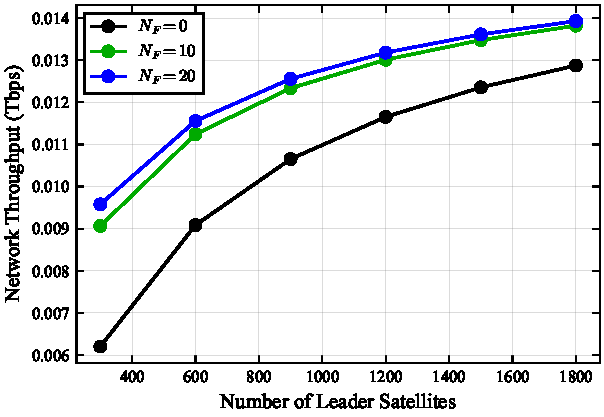
\includegraphics[width=0.78\linewidth]{../figures/interference/figI4_network_throughput.pdf}
    \caption{网络总吞吐随 leader 数量变化。}
    \label{fig:i4}
\end{figure}

图 \ref{fig:i4} 使用
\[
    T_{\rm net}=N_{\rm L}\bar R_{\rm cl}^{\rm I}
\]
计算网络总吞吐。随着 $N_{\rm L}$ 增加，网络吞吐仍缓慢上升，说明更多 cluster 带来的
空间复用增益没有完全消失。然而曲线增幅明显趋缓：以 $N_{\rm F}=20$ 为例，
$N_{\rm L}$ 从 $300$ 增至 $1800$ 时，吞吐从约 $0.0096$ Tbps 增至约 $0.0139$
Tbps，远低于无干扰直觉下的线性扩展。

因此，密集网络中继续增加 leaders 或 followers 的收益需要用全网吞吐和覆盖约束共同
评价。若只看 $T_{\rm net}$，高密度可能仍略有收益；若加入 Fig.I2 的 coverage 约束，
这种收益会伴随显著可靠性损失。

\section{Fig.I5：二维参数面与推荐区域}

\begin{figure}[htbp]
    \centering
    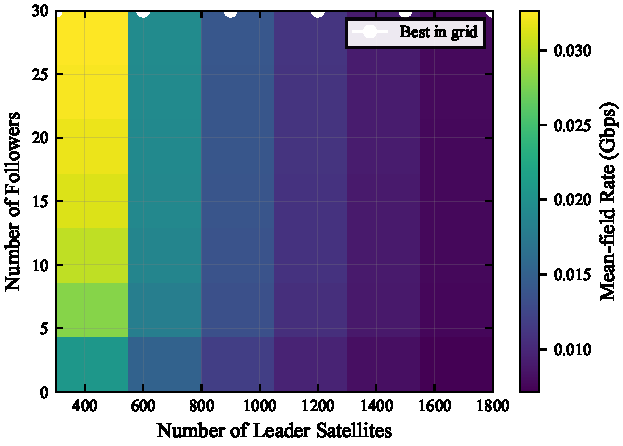
\includegraphics[width=0.78\linewidth]{../figures/interference/figI5_nf_nl_heatmap.pdf}
    \caption{$N_{\rm L}$--$N_{\rm F}$ 二维参数面上的均值场 cluster rate。白线标出扫描网格内的最大速率点。}
    \label{fig:i5}
\end{figure}

图 \ref{fig:i5} 显示，在本参数范围和仅以平均 cluster rate 为目标时，扫描网格中的
最优点倾向于选择更大的 $N_{\rm F}$，但颜色变化同时说明平均速率随 $N_{\rm L}$ 增加
明显下降。这个结论需要谨慎解释：白线表示的是“给定 $N_{\rm L}$ 后、在扫描范围内平均
速率最高的 $N_{\rm F}$”，不是无条件推荐高 follower 密度。

结合 Fig.I2 可得到更稳健的工程建议：若系统目标是低阈值、尽力而为的数据吞吐，可以
使用较多 followers 来获得有限的中继增益；若目标包含中等 SINR threshold 或 outage
约束，应限制每个 cluster 的 followers 数量，或者引入频率复用、波束协调、功率控制、
用户调度等干扰管理机制。

\section{综合结论}

本扩展研究得到三点结论。

第一，原复现模型中的 follower 增益在噪声受限条件下成立，但在密集同频网络中会被
集群间干扰显著削弱。继续增加 followers 不只增加服务分支，也会等比例增加其他
clusters 的可见干扰源。

第二，在同频全复用假设下，SINR coverage 比平均速率更敏感。即便平均 cluster rate
随 $N_{\rm F}$ 仍有小幅上升，coverage 曲线已经明显左移，说明系统可靠性先于平均吞吐
成为瓶颈。

第三，密集 follower-based LEO 网络的合理设计不应只优化单集群速率，而应联合优化
$N_{\rm L}$、$N_{\rm F}$、频率复用、波束隔离与调度策略。若不进行干扰协调，增加
followers 的主要收益会从“线性速率提升”变成“低 SINR 区域的有限补偿”，难以支撑
高可靠覆盖目标。

\end{document}
